\chapter{Ergebnisse}
\label{ch:Ergebnisse}

\section{Phase 1: REE}

\section{Phase 2: IEEE 39 Bus System}
\subsection{Small-Signal Stability Result}


\subsection{Evolution of the Dominant System Modes}

The evolution of the dominant system modes was evaluated for increasing photovoltaic (PV) penetration levels in the modified IEEE 39-bus system. The penetration level was gradually increased by replacing synchronous generators with converter-based generation, resulting in the scenarios R00–R07.

Table \ref{tab:dominant_modes} summarizes the dominant eigenvalue identified for each operating condition. The table includes the eigenvalue location, the corresponding oscillation frequency, and the damping ratio of the dominant mode.

\begin{table}[h]
\centering
\caption{Dominant system modes for increasing PV penetration}
\label{tab:dominant_modes}
\begin{tabular}{ccccc}
\hline
Case & Dominant Mode & Eigenvalue $\sigma + j\omega$ [1/s] & Frequency [Hz] & Damping [\%] \\
\hline
R00 & Mode 00005 & $-0.197 + j6.975$ & 1.110 & 2.82 \\
R01 & Mode 00017 & $-0.384 + j6.613$ & 1.052 & 5.80 \\
R02 & Mode 00021 & $-0.384 + j6.739$ & 1.072 & 5.69 \\
R03 & Mode 00019 & $-0.382 + j6.735$ & 1.072 & 5.67 \\
R04 & Mode 00033 & $-0.461 + j7.550$ & 1.202 & 6.10 \\
R05 & Mode 00027 & $-0.381 + j6.244$ & 0.994 & 6.10 \\
R06 & Mode 00031 & $-0.407 + j6.535$ & 1.040 & 6.22 \\
R07 & Mode 00001 & $+59.464$ & -- & Unstable \\
\hline
\end{tabular}
\end{table}

The results show that the dominant modes remain located in the left half of the complex plane for scenarios R00–R06, indicating that the system remains locally stable around the operating point. The oscillatory modes are located around approximately 1 Hz, which is consistent with typical electromechanical oscillations observed in large interconnected power systems.

Across the different scenarios, the damping ratio of the dominant mode remains relatively stable, ranging approximately between 5\% and 6\%. Overall, the eigenvalue analysis indicates that increasing PV penetration up to scenario R06 does not significantly degrade the small-signal stability of the system, as the dominant oscillatory modes remain well damped and located in the left half of the complex plane.

\begin{figure}[htbp!]
    \centering
    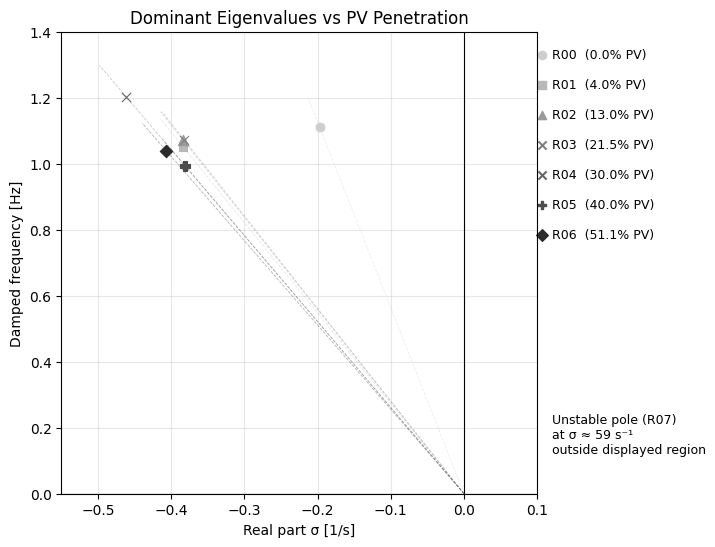
\includegraphics[width=0.8\textwidth]{Figures/Chapter 7/Dominant Modes vs PV Penetration.png}
    \caption{Dominant modes with respect to PV penetration level}
    \label{fig:dominant modes vs pv penetration}
\end{figure}

\subsubsection{Dynamic Feasibility of the Operating Point}

Although the small-signal stability analysis indicates stable operating points up to scenario R06, time-domain RMS simulations reveal a different behavior when disturbances are applied.

Table \ref{tab:rms_feasibility} summarizes the feasibility of RMS dynamic simulations for the analyzed scenarios.

\begin{table}[h]
\centering
\caption{RMS simulation feasibility for increasing PV penetration}
\label{tab:rms_feasibility}
\begin{tabular}{cccc}
\hline
Case & PV Penetration & RMS (No Event) & RMS (With Fault) \\
\hline
R05 & $\sim$40\% & $\checkmark$ & $\checkmark$ \\
R06 & $\sim$51\% & $\checkmark$ & $\times$ \\
R07 & $\sim$62\% & $\times$ & $\times$ \\
\hline
\end{tabular}
\end{table}

The results show that scenario R06 can still maintain the operating point when no disturbance is applied. However, when a severe disturbance such as a three-phase fault is introduced, the RMS simulation fails to converge. This behavior indicates that the system has already lost robustness against large disturbances, even though the operating point remains locally stable according to the small-signal analysis.

\subsubsection{Emergence of an Unstable Mode}

In scenario R07, the system becomes unstable even in the absence of disturbances. The eigenvalue analysis reveals the appearance of a positive real eigenvalue, indicating loss of small-signal stability.

The participation factor analysis of this unstable mode shows that it is dominated by internal states associated with the phase-locked loop (PLL) of the converter-based generation models. In particular, the highest participation factors correspond to the PLL internal states responsible for phase estimation and synchronization.

\begin{figure}[htbp!]
    \centering
    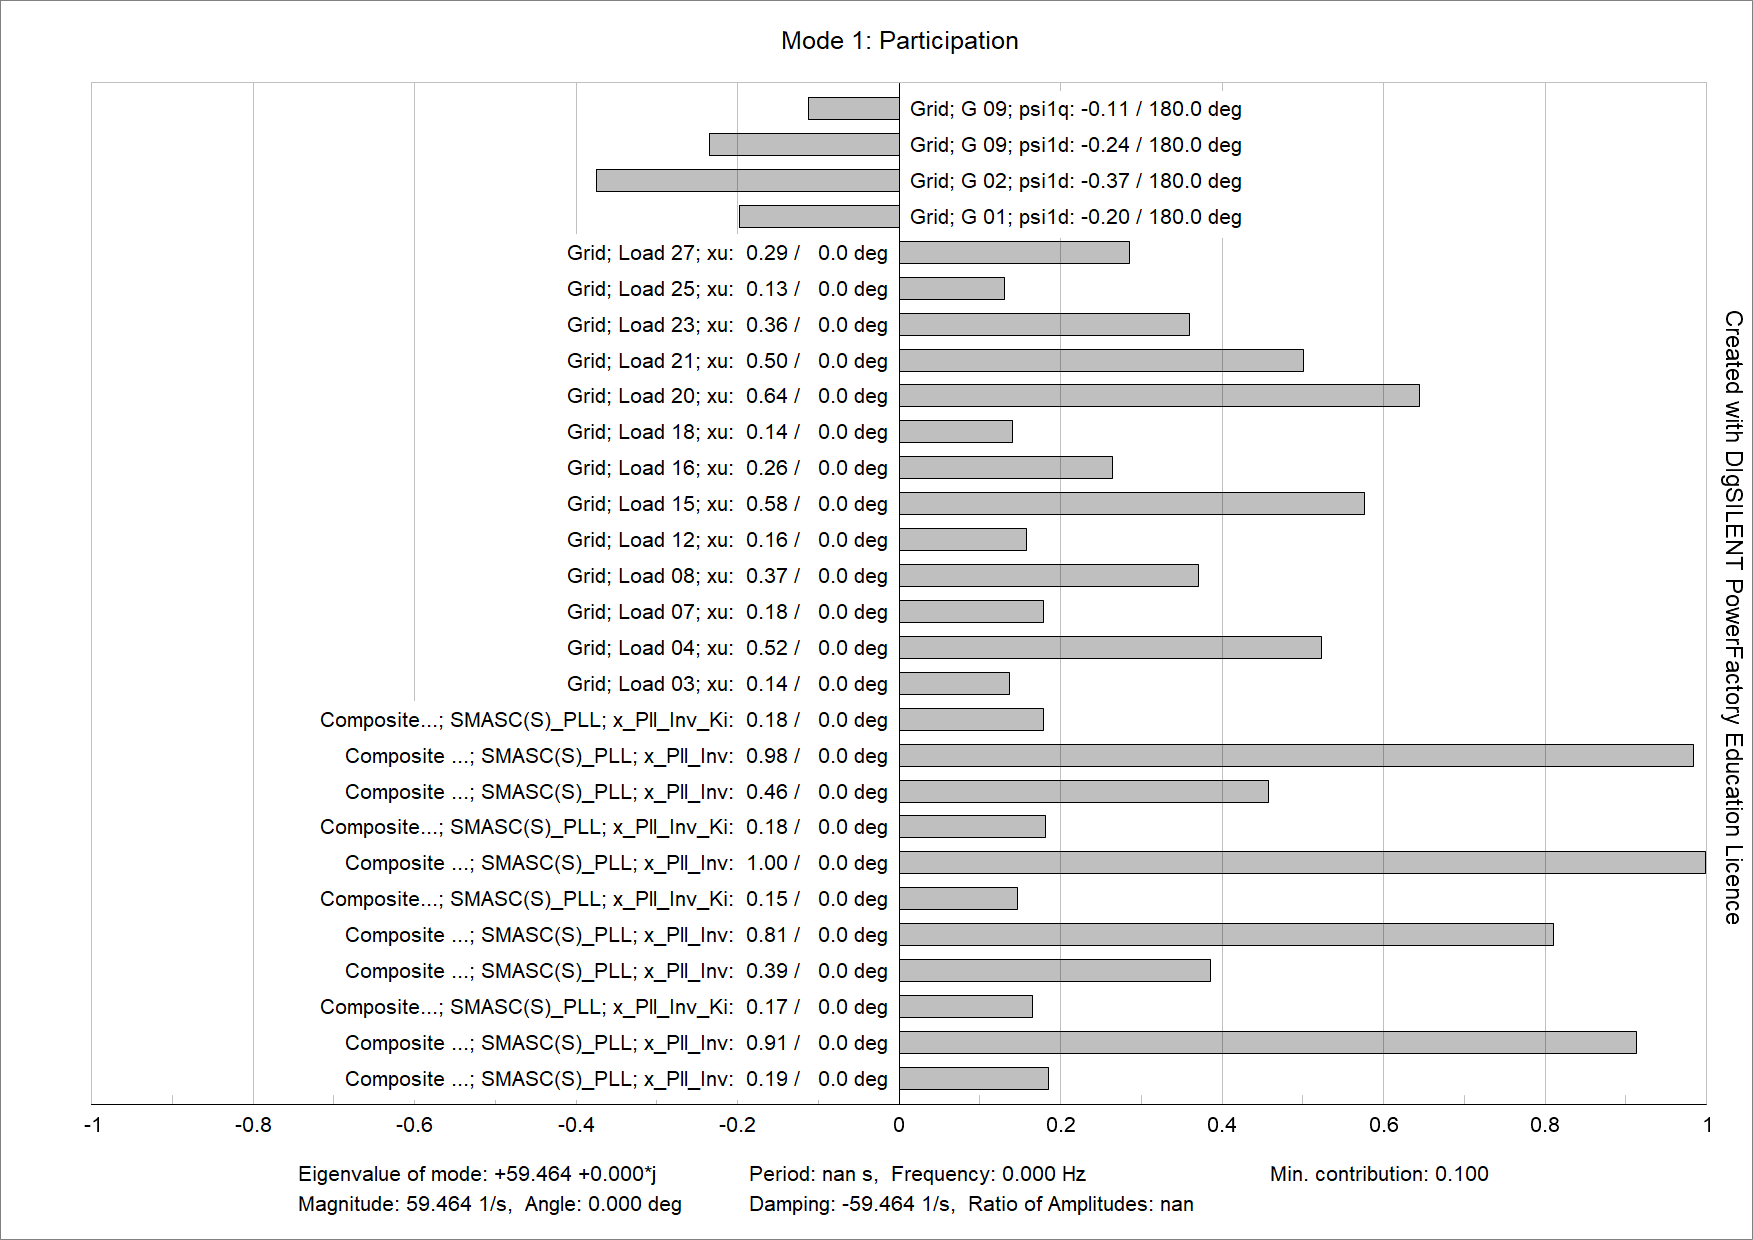
\includegraphics[width=0.8\textwidth]{Figures/Chapter 7/Mode Dominant Unstable R07.png}
    \caption{ticipation factors of the unstable mode identified in scenario R07.}
    \label{fig:participation_unstable_mode}
\end{figure}
Several network states also contribute to the mode, indicating that the instability results from an interaction between converter control dynamics and the surrounding power system.

This behavior suggests that at very high penetration levels, grid-following converters struggle to maintain a stable synchronization reference due to the reduced presence of synchronous machines in the system.

\subsubsection{Summary of Observed Stability Limits}

Based on the performed analysis, two stability limits can be identified:

\begin{itemize}
\item \textbf{Dynamic robustness limit}: between scenarios R05 and R06, where the system begins to lose the ability to withstand large disturbances in time-domain RMS simulations.

\item \textbf{Small-signal stability limit}: between scenarios R06 and R07, where an unstable eigenvalue appears and the operating point itself becomes unstable.
\end{itemize}

These results highlight the increasing influence of converter control dynamics in systems with high shares of converter-based generation.